\documentclass{bioinfo}

\usepackage{multicol} % Merge cells horizontally
\usepackage[pdfborder={0 0 0}]{hyperref} % links, but no colored boxes
\hypersetup{breaklinks=true,
pagecolor=white,
colorlinks=false,}
\urlstyle{rm} %so it doesn�t use a typewriter font for url�s.

\hyphenation{BioPax BioCarta PaxTools}
% Useful macros:
\newcommand{\TTra}{\textsuperscript{\tiny{\texttrademark}\,}}
\newcommand{\qual}{\texttt{qual}}



\copyrightyear{2012}
\pubyear{2012}

\begin{document}

\firstpage{1}

\title[BioPax to SBML qual]{Qualitative translation of relations from BioPax to SBML qual}
\author[Finja B\"uchel \textit{et~al}]{Finja B\"uchel\,$^{1\footnote{to whom correspondence should be addressed}}$, and Andreas Zell\,$^1$}

\address{$^{1}$Center for Bioinformatics Tuebingen (ZBIT), \\University of Tuebingen, 72076 T\"ubingen, Germany}
\history{Received on XXXXX; revised on XXXXX; accepted on XXXXX}

\editor{Associate Editor: XXXXXXX}

\maketitle

\begin{abstract}

\section{Motivation:}
The Biological Pathway Exchange Language (BioPax) and the Systems Biology Markup Language (SBML) are the two most popular modeling and data exchange languages in systems biology.
The focus of SBML is quantitative modeling and dynamic simulation of molecular interaction pathways, whereas the BioPax specification concentrates on visualization and qualitative analysis of pathway maps.
BioPax describes reactions and relations. In contrast, reactions are the only type of interaction in core SBML.
With the release of the SBML Qualitative Models extension (\qual), it has recently also become possible to describe relations in SBML.
Before this release, relations could not be translated to SBML or were erroneously converted to reactions. Until now, there exists no BioPax to SBML converter that is fully capable to translate both reactions and relations.
\section{Results:}
Here we present the conversion result of the complete nature Pathway Interaction Database (PID), which includes pathways from BioCarta, Reactome, and from the National Cancer institute.
All PID BioPax Level~2 and Level~3 pathway files have been translated to the SBML format including both reactions and relations by using the new \qual{} extension package.
\section{Availability:}
The complete collection of the PID models is freely available on our homepage ..... (\textbf{TODO Finja: create homepage! and and if necessary licence})
\section{Contact:} \href{finja.buechel@uni-tuebingen.de}{finja.buechel@uni-tuebingen.de}
\end{abstract}

\section{Introduction}
The goal of systems biology is the model-driven understanding of biological and chemical processes across the scale in detailed levels.
The Biological Pathway Exchange Language (BioPax) and the Systems Biology Markup Language (SBML) are common modeling languages that facilitates the exchange and storage of in-silico models.
The BioPax specification aims at exchanging, visualization, and analyzing such processes on a large scale.
BioPax can be used to image metabolic, signaling, molecular, gene regulatory and genetic interaction networks \citep{Demir2010}.
In contrast, SBML is mostly used for quantitative modeling because it offers the possibility to include kinetic equations and enables the interpretation of the interaction network as an differential equation system \citep{Hucka2003}.
The SBML core specification defines reactions in detail but no other relationships between molecules.
%problem
Before the release of the Qualitative Models specification (\qual, \citealp[see][]{QualSpecification}), it was not possible to define relations or to integrate reactions and relations in one model.
%relevance
Furthermore, the combination or exchange of information between different databases if one database uses the BioPax format and the other one the SBML format was difficult or even impossible.
%literature review
So far, there exist several visualization tools, like Cytoscape or CellDesigner, which can handle both formats by using plugins \citep{Mi2011, Funahashi2007, Smoot2011a, Zinovyev2008}).
\citet*{Ruebenacker2009} suggest a new a bridging format to solve the problem of the conversion from BioPax to SBML.
But until now, there exists mainly converters from SBML to BioPax like \emph{The System Biology Format Converter} \citep[see][]{SBFC} but no converter for BioPax to SBML, whose conversion would also include relations.
The need to combine both formats to use the knowledge from a multitude of databases in various application becomes more and more urgent.

% what we did
% necessary to mention why we use PID?
In this paper we present a complete conversion of the nature Pathway Interaction Database (PID, \citet{Schaefer2009}) from BioPax Level~2 and Level~3 format to the SBML format including the \qual{} extension.
The pathway conversion is implemented in Java\TTra and uses JSBML \citep{Draeger2011} and PaxTools \citep{Demir2010}.
The translated files are freely available on our homepage: ...\textbf{TODO and add licence}
% what we find out?
% what do the results mean (why are they significant?)


\begin{methods}
\section{Material and Methods}
\subsection{The SBML and the Qualitative Models extension}
%%%%%%%%% SBML
The SBML (Systems Biology Markup Language) core specification defines a special XML dialect to describe quantitative models.
Therefore, several classes are defined describing reactive species and their interaction in a model.
The most important classes are \texttt{species} and \texttt{reaction}.
A \texttt{species} element can describe each kind of molecule and can be further determined with the aid of MIRIAM annotations \citep{Novere2005}.
The SBML core specification provides no possibility to define other relationships than concrete quantitative reactions \citep{Hucka2003}.

%%%%%%%%% SBML qual
The SBML Qualitative Models extension (\qual) introduces qualitative elements, such as \texttt{qualitativeSpecies}, \texttt{symbol}, and \texttt{transition}, providing the necessary means to describe relationships like enzyme-enzyme relations, protein-protein interactions, interactions of transcription factors and genes, protein-compound interaction, or links to other pathways.
%Although, technically, those processes are chemical reactions, too, it can often be far more useful to represent them by logical states and transitions.
Instead of concentration levels that are transformed continuously via reactions, \texttt{qualitativeSpecies} have discrete states that are changed using \texttt{transition}s.
These \texttt{transitions} consist of \texttt{input} and \texttt{output} elements and at least one \texttt{functionTerm}.
If, in a qualitative model, protein A inhibits protein B, this would be represented as a \texttt{transition} with \texttt{input} A having the \texttt{sign} attribute "negative" and \texttt{output} B.
The \texttt{sign} attribute of the \texttt{input} elements describes if the relationship between the input and output elements is \emph{positive}, \emph{negative}, \emph{dual}, or \emph{unknown}. \emph{Dual} means that the transition can operate both activating (\emph{active}) and inhibiting (\emph{negative}). In contrast, \emph{unknown} is assigned to the \texttt{Input} if the transition effect is not further specified.
\subsection{The BioPax specification}
The Biology Pathway Exchange Language (BioPax) is an OWL (Web Ontology Language) dialect which based on the RDF syntax.
There is one super class called \texttt{entity} which extends all other BioPax classes.
 Two main classes are distinguished: \texttt{PhysicalEntity} and \texttt{Interaction}.
\texttt{PhysicalEntity} describes molecules, like proteins, complexes, small molecules, DNA, or RNA, whereas \texttt{Interaction} defines reactions and relations between the \texttt{PhysicalEntity}'s.
\texttt{Interaction} is split into \texttt{Control} and \texttt{Conversion}
which can be separated into the subclasses \texttt{Catalysis}, \texttt{Modulation}, \texttt{Transport}, \texttt{BiochemicalReaction}, and \texttt{Complex\-Assembly}.

BioPax is released level-wise.
The current level is Level~3.
Level 1 is exclusively able to describe metabolic interactions, whereas Level~2 supports signaling pathways and molecular interactions.
In addition to Level~2, gene regulatory networks and genetic interactions can be described with Level~3.
For this purpose the \texttt{Control} subclass \texttt{TemplateReactionRegulation} and the \texttt{Conversion} subclass \texttt{Degradation} have been added.
Furthermore, \texttt{PhysicalEntity} is now able to define \texttt{DNAregion} and \texttt{RNAregion}.
Level~3 is not backwards compatible with Level~2, but Level~2 is backwards compatible with Level 1 \citep{Demir2010}.
In this paper all BioPax element names begin with capital letters and refer to Level~2 and 3.
Otherwise it is explicitly denoted in the text.
\subsection{Implementation}
The conversion was programmed with Java\TTra, using JSBML \citep{Draeger2011} with the Qualitative Models extension, PaxTools, and the KEGG API \citep{Kanehisa2006}.
PaxTools was used to read the BioPax files and to manipulate the information content.
This information was extended with MIRIAM identifiers for the following databases: Entrez Gene, Omim, Ensembl, UniProt, ChEBI, DrugBank, Gene Ontology, HGNC, PubChem, 3DMET, NCBI Taxonomy, PDBeChem, GlycomeDB, LipidBank, EC-Numbers (enzyme nomeclature) and various KEGG databases (gene, glycan, reaction, compound, drug, pathway, orthology)\citep{Novere2005}.

\subsection{Conversion of BioPax to SBML \qual}\label{subsec:BioPax}
%%%%%%%%%%%%%%%%%%%%%%%%%%% FIGURE 1 %%%%%%%%%%%%%%%%%%%%%%%%%%%%%%%%%%%%%%%%%%%%%%%%%%
\begin{figure*}[t!h]
\centering 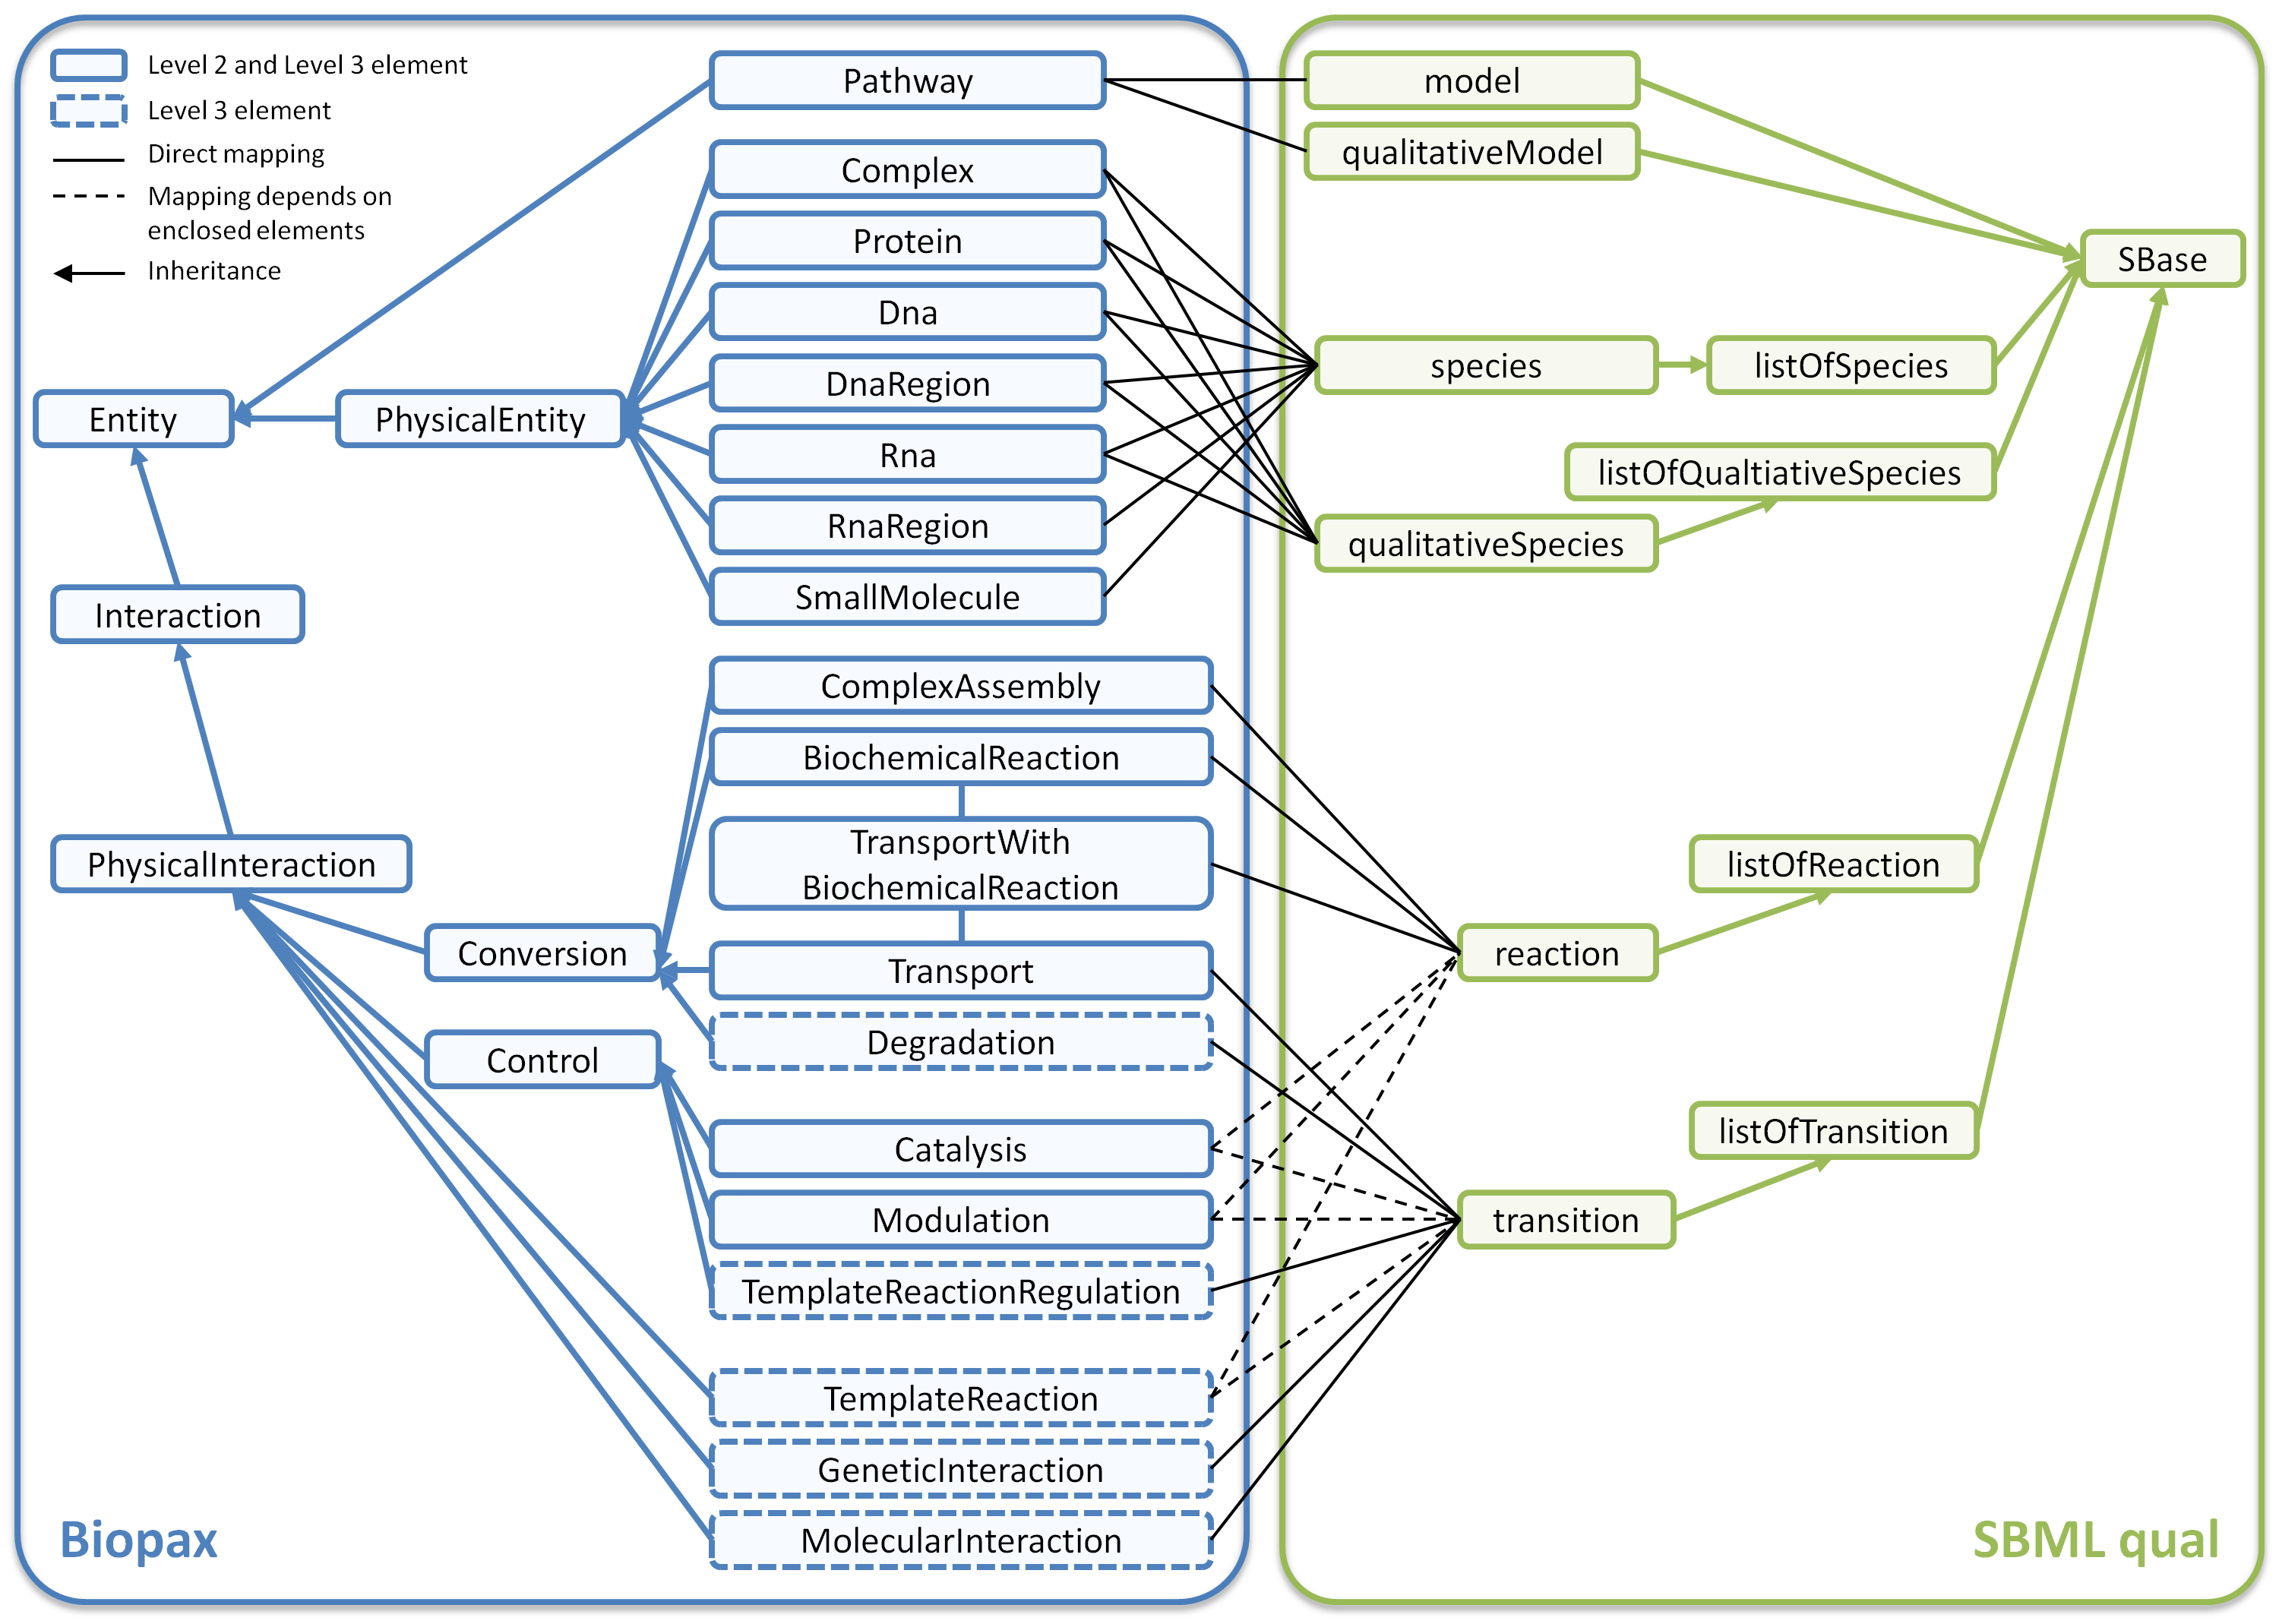
\includegraphics[width=0.95\textwidth]{BioPaxSBMLqual.png}
\caption{Conversion from BioPax Level~2 and Level~3 to SBML with the Qualitative Models extension (\qual).
The green rounded rectangles describe the SBML and SBML \qual{} classes, and the blue ones the BioPax elements.
The distinction between BioPax Level~2 and Level~3 elements is visualized with dashed rectangles.
These dashed rectangles denote Level~3 elements which are not available in Level~2.
All other elements occur in both levels.
The ancestry of both BioPax and SBML elements is drawn as blue arrows for BioPax respectively with green arrows for SBML.
The conversion from BioPax to SBML \qual{} is drawn with black lines.
For some BioPax elements, it depends on the enclosed entities if the BioPax element is translated to a reaction or to a relation.
This translation dependency is visualized with black dashed lines.
A detailed translation description of these elements is shown in Table~\ref{Tab:BioPax2SBML}.}
\label{fig:BioPaxSBMLqual}
\end{figure*}
%%%%%%%%%%%%%%%%%%%%%%%%%%% END FIGURE 1 %%%%%%%%%%%%%%%%%%%%%%%%%%%%%%%%%%%%%%%%%%%%%%
The complete nature Pathway Interaction Database (PID) is converted from BioPax to SBML including the Qualitative Models extension.
PID provides curated pahtways from the National Cancer Institute, pathways from BioCarta from June 2004, and human Reactome pathways (Version 22), whereas the Reactome data is updated as soon as new pathway information is available \citep{Schaefer2009}.
The translation of the BioPax Level~2 and Level~3 pathway files is performed in five steps.
An overview of the mapping from BioPax elements to SBML and to SBML \qual{} elements is shown in Figure~\ref{fig:BioPaxSBMLqual}.

%%%%%%%%%%%%%% 1. Step %%%%%% determine organism
In the first step, the pathway organism is determined by searching for the BioSource reference in the BioPax file.
The default organism is human.

%%%%%%%%%%%%%% 2. Step %%%%%% model creation
In the second step, the SBML \texttt{model} and \texttt{qualitativeModel} are build.
The models correspond to the complete pathway represented in the BioPax file.

%%%%%%%%%%%%%% 3. Step %%%%%% entities and annotation
% conversion of Entities, gene id...
In the third step, for each \texttt{PhysicalEntity} a SBML \texttt{species} and \texttt{qualitativeSpecies} is created.
Depending of the kind of the \texttt{PhysicalEntity}, i.e. if it is a protein, complex, DNA, RNA, or small molecule, the species is annotated with the corresponding SBO term (\citealp{SBO}, see Table~\ref{Tab:BioPax2SBO} for a list of used terms).

%%%%%%%%%%%%%%%%%%%%%%%%%%% TABLE X %%%%%%%%%%%%%%%%%%%%%%%%%%%%%%%%%%%%%%%%%%%%%%%%%
\begin{table}[tb]
\processtable{BioPax entities and assigned SBO terms\label{Tab:BioPax2SBO}}
{\begin{tabular}{llll}\toprule
\textbf{BioPax entity} & \textbf{Assigned SBO term} & \textbf{SBO name} \\
\midrule
Complex         & SBO:0000253 & non-covalent complex \\
Protein         & SBO:0000252 & polypeptide chain \\
Dna             & SBO:0000251 & deoxyribonucleic acid \\
DnaRegion       & SBO:0000251 & deoxyribonucleic acid \\
Rna             & SBO:0000250 & ribonucleic acid \\
RnaRegion       & SBO:0000250 & ribonucleic acid \\
SmallMolecule   & SBO:0000247 & simple chemical \\
Gene            & SBO:0000240 & informational molecule segment \\
\botrule
\end{tabular}}
{
Each BioPax \texttt{Entity} is converted to a SBML \texttt{species} and \texttt{qualitativeSpecies}.
In BioPax, one can specify the nature of the real entity by classes, that are derived from \texttt{Entity} (e.g., DNA, Protein, etc).
SBML does not contain specific entities that can be derived from a SBML \texttt{species}.
The common way to separate different genomic entities in SBML is using SBO terms from the material entity branch.
This table specifies the SBO terms that we used to distinguish between various cellular entities in SBML.
}
\end{table}
%%%%%%%%%%%%%%%%%%%%%%%%%%%%%%%%%%%%%%%%%%%%%%%%%%%%%%%%%%%%%%%%%%%%%%%%%%%%%%%%%%%%%

% CW: Compartment text ist IMHO nicht richtig und unwichtig => entfernt.
%Then the \texttt{species}' compartment is assigned depending on the GO annotation of the \texttt{PhysicalEntity}.
%If no GO term is specified the \texttt{species} is assigned to a default compartment.

Finally, the BioPax document is mined for an RDF link from the \texttt{PhysicalEntity} to a corresponding Entrez Gene ID. These identifers are unique and facilitates the automated annotation of this species (described in the fifth step).
If there exists no Gene ID but a gene symbol, the gene symbol is mapped to a Gene ID. \textbf{TODO: Clemens das noch n\"aher ausf\"uhren?}
If neither a Gene ID nor a gene symbol is available the name of the \texttt{PhysicalEntity} is used.


%%%%%%%%%%%%%% 4. Step %%%%%% reaction relations
In the fourth step, the BioPax interaction elements are converted.
Interaction elements can be split in \texttt{Conversion} and \texttt{Control} elements.

\texttt{Conversion}s are mainly translated into SBML reactions except of the \texttt{Transport} and the \texttt{Degradation} elements, which are translated into transitions. Translation of reactions from BioPax to SBML is performed by creating the same reaction with all substrates, products and enzymes in SBML. Furthermore BioPax Level~3 provides the stoichiometry of the reactants and products of \texttt{BiochemicalReaction}s and \texttt{TransportWithBiochemicalReaction}s which are also translated to SBML.Level~2 does not provide stoichiometric information.

The conversion of the \texttt{Control} elements is straightforward, whereas the conversion of \texttt{Control} elements is more sophisticated, because translation into a transition or a reaction depends on the enclosed \texttt{Control} elements.
\texttt{Control} elements always consist of zero or more \texttt{Controller} and zero or one \texttt{Controlled} elements.
\texttt{Controller} elements can be inherited from \texttt{PhysicalEntity} or \texttt{Pathway}, whereas \texttt{Controlled} elements are also \texttt{Interaction} elements.
Thus, it depends on the kind of \texttt{Controller} and the \texttt{Controlled} element if the \texttt{Interaction} is translated to a SBML reaction or transition.
If the \texttt{Controller} or the \texttt{Controlled} element is a \texttt{Pathway} element the \texttt{Interaction} is always converted to a transition, because in biology it is not possible to create a reaction with a complete pathway as an reactant or a product.
A \texttt{Conversion} is translated into a \texttt{transition} if the \texttt{Controlled} element is translated to a transition, too.
For instance, the conversion of a \texttt{Modulation}, consisting of a \texttt{PhysicalEntity} as \texttt{Controller} and a \texttt{BioChemicalReaction} as \texttt{Controlled}, is translated to a reaction.
An example is shown in Figure~\ref{fig:Ceramide} which shows the ceramide signaling pathway, where the biochemical reaction from sphingomyelin to ceramide (the \texttt{Controlled} element) is positively modulated from SMPD1+ (the \texttt{Controller}).
This modulation will be converted into a reaction where SMPD1+ is modelled as an enzyme of the reaction.
But if the \texttt{Controlled} element is a \texttt{Degradation}, the \texttt{Modulation} is converted into a transition.
In some cases, the \texttt{Controlled} element is an \texttt{Interaction} entity that does not belong to a special subclass.
Then, the \texttt{Controlled} element itself is translated into a transition, and the connection between the \texttt{Controller} and the translated transition is also translated into a transition.
The \texttt{sign} attribute of the \texttt{Input} element is determined depending on the \texttt{ControlType} attribute. This attribute is assigned to nearly all \texttt{Control} elements. If the \texttt{ControlType} is activating \texttt{sign} is set to\emph{active}, if it is inhibiting \texttt{sign} is set ton\emph{negative}, if it is both \texttt{sign} is set to \emph{dual}, and otherwise \texttt{sign} is set to \emph{unknown}.
A detailed overview of the conversion of the \texttt{Control} elements is shown in Table~\ref{Tab:BioPax2SBML}.

%%%%%%%%%%%%%%%%%%%%%%%%%%% TABLE 1 %%%%%%%%%%%%%%%%%%%%%%%%%%%%%%%%%%%%%%%%%%%%%%%%%
\begin{table}[t!h]
\processtable{Description of the translation of BioPax \texttt{Control} elements\label{Tab:BioPax2SBML}}
{\begin{tabular}{llll}\toprule
BioPax controller & BioPax controlled               & Converted\\
                  &                                 & SBML \qual\\
                  &                                 & element\\
\midrule
%\textbf{BioPax Level~3}\\
\multicolumn{3}{c}{\centering \textbf{BioPax Level~3}}\\
\midrule
PhysicalEntity & BiochemicalReaction                & reaction\\
PhysicalEntity & ComplexAssembly                    & reaction\\
PhysicalEntity & Conversion                            & transition\\
PhysicalEntity & Degradation                        & transition\\
PhysicalEntity & Transport                          & transition\\
PhysicalEntity & TransportWithBiochemicalReaction   & reaction\\
PhysicalEntity & Pathway                            & transition\\
PhysicalEntity & TemplateReaction                   & transition\\
\\
Pathway         & BiochemicalReaction               & transition\\
Pathway         & ComplexAssembly                   & transition\\
Pathway         & Conversion                        & transition\\
Pathway         & Degradation                       & transition\\
Pathway         & Pathway                           & transition\\
Pathway         & TemplateReaction                  & transition\\
Pathway         & Transport                         & transition\\
Pathway         & TransportWithBiochemicalReaction  & transition\\
\\\midrule
%\textbf{BioPax Level~2}\\
\multicolumn{3}{c}{\centering \textbf{BioPax Level~2}}\\
\midrule
physicalEntity & biochemicalReaction                & reaction\\
physicalEntity & complexAssembly                    & reaction\\
physicalEntity & interaction                        & transition\\
physicalEntity & pathway                            & transition\\
physicalEntity & transport                          & transition\\
physicalEntity & transportWithBiochemicalReaction   & reaction\\
\\
pathway         & biochemicalReaction               & transition\\
pathway         & complexAssembly                   & transition\\
pathway         & interaction                       & transition\\
pathway         & pathway                           & transition\\
pathway         & transportWithBiochemicalReaction  & transition\\
pathway         & transport                         & transition\\\botrule
\end{tabular}}{BioPax \texttt{Control} elements consists of a \texttt{Controller} and one or more \texttt{Controlled} elements.
Depending on the kind of \texttt{Controller} or \texttt{Controlled} element, the \texttt{Control} entity is translated to an SBML reaction or transition.
The table gives an overview of this conversion regarding BioPax Level~2 and BioPax Level~3. The Level~2 entities are labeled with small initial letters and the translation is listed in the lower part of the table.}
\end{table}
%%%%%%%%%%%%%%%%%%%%%%%%%%% END TABLE 1 %%%%%%%%%%%%%%%%%%%%%%%%%%%%%%%%%%%%%%%%%%%%%%%

%%%%%%%%%%%%%%%% Step 5 %%%%% annotation %%%%%%%%
%% CLEMENS: MIRIAM und SBO                     %%
%%%%%%%%%%%%%%%%%%%%%%%%%%%%%%%%%%%%%%%%%%%%%%%%%
In the fifth and final step, the SBML instances are further annotated.
The BioPax specification allows users to encode arbitrary identifiers for elements.
These can be identifiers for various databases, e.g., UniProt, Entrez Gene, Ensembl, etc. Unfortunately, the syntax used in BioPax is sometimes inconsistent which leads to XML database annotations like "UniProt" or "UniProtKB" within BioPax documents that hamper the automatic reading and interpretation of those models by third party applications.
%%%%%%%%%%% Beispiel %%%%%%%%%%%%%%%%%%%%
%  <bp:unificationXref rdf:ID="unificationXref14">
%    <bp:DB rdf:datatype="http://www.w3.org/2001/XMLSchema\#string">UniProt</bp:DB>
%    <bp:ID rdf:datatype="http://www.w3.org/2001/XMLSchema\#string">Q4KMY3</bp:ID>
%  </bp:unificationXref>
%  <bp:unificationXref rdf:ID="unificationXref14">
%    <bp:DB rdf:datatype="http://www.w3.org/2001/XMLSchema\#string">UniProtKB</bp:DB>
%    <bp:ID rdf:datatype="http://www.w3.org/2001/XMLSchema\#string">Q4KMY3</bp:ID>
%  </bp:unificationXref>
%  <bp:unificationXref rdf:ID="unificationXref14">
%    <bp:DB rdf:datatype="http://www.w3.org/2001/XMLSchema\#string">UniProt</bp:DB>
%    <bp:ID rdf:datatype="http://www.w3.org/2001/XMLSchema\#string">Q4KMY3, Q7Z5L2</bp:ID>
%  </bp:unificationXref>
%%%%%%%%%%% Beispiel ENDE %%%%%%%%%%%%%%%%%%%%

In SBML, such identifiers can be expressed as standardized MIRIAM URNs that can be added as annotation to any SBML element.
We support and add MIRIAM identifiers for the following databases: Entrez Gene, Omim, Ensembl, UniProt, ChEBI, DrugBank, Gene Ontology, HGNC, PubChem, 3DMET, NCBI Taxonomy, PDBeChem, GlycomeDB, LipidBank, EC-Numbers (enzyme nomeclature) and various KEGG databases (gene, glycan, reaction, compound, drug, pathway, orthology). To obtain identifiers for those databases, we map the Entrez Gene identifier, which we annotated on every element in Step 2, to a KEGG identifier. Using the KEGG API, we then query all of those identifiers to retrieve better names, descriptions and the mentioned database identifiers.
%CW: Entfernt. wurde durch neuen satz (s.o.) ersetzt.
%All supported identifiers from the BioPax files are parsed, some are manually curated by us, and some annotations are supplemented by additional queries to the KEGG API for every translated element.
The goal of those annotations is to provide models that can be used directly by many researchers, no matter what identifiers or databases they use.
\end{methods}


\section{Results and Discussion}
%http://pid.nci.nih.gov/about.shtml#pid
% TODO: das ist der Link, der unbedingt in die �bersetzten die Pathways geschrieben werden muss.
%%%%%%%%%%%%%%%%%%%%%%%%%%% BEGIN FIGURE 2 %%%%%%%%%%%%%%%%%%%%%%%%%%%%%%%%%%%%%%%%%%%%%
\begin{figure}[t!h]
\centering 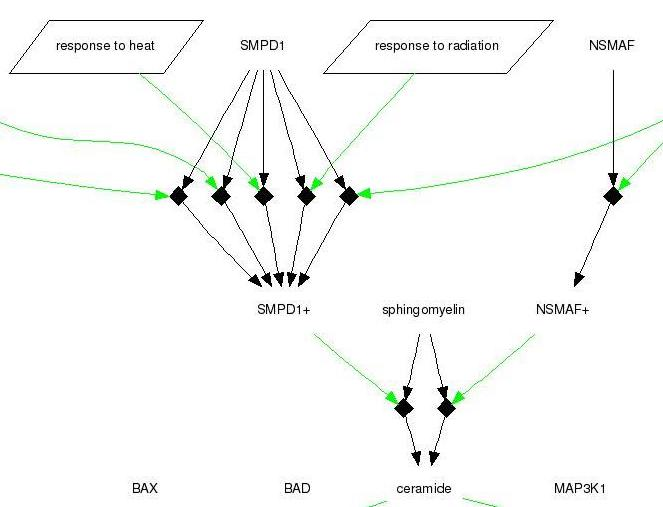
\includegraphics[width=0.95\columnwidth]{CeramidePart.jpg}
\caption{Part of the ceramide signaling pathway imported from BioCarta into the Pathway Interaction Database (PID).
Modifications are denoted with black diamonds.
The entities with an black arrow to the diamond desribe the modulation inputs and the entities with an black arrow out of the diamond the modulation output.
The green arrows symbolize positive regulators and the round rectangles complexes.
Pathways are visualized with a trapezium.
The website of the National Cancer Institute (http://www.cancer.gov) \textbf{TODO: Laut homepage soll der Link so angegeben werden. Ist das richtig?}}
\label{fig:Ceramide}
\end{figure}
%%%%%%%%%%%%%%%%%%%%%%%%%%% END FIGURE 2 %%%%%%%%%%%%%%%%%%%%%%%%%%%%%%%%%%%%%%%%%%%%%%%
%Aufbau:
%Kern problem: BioPax-Format der PID Pathways und die fehlende M�glichkeit relationen darzustellen.
%1. PID ist toll weil...
%2. Man k�nnte so viel tun (Simulation, Informationsverkn\"upfung
%3. Aber das Format ist ungeeignet
%4. Daher gibt es mehrere Konverter, die folgendes k�nnen reaction
%5. Das gen�gt nicht weil wir brauchen relationen
%6. Jetzt gibt es endlich BioPax to SBML qual, das viel besser ist weil,...
%7. Im folgenden werden die Merkmale n�her erl�utert.

The Pathway Interaction Database (PID) is a curated and peer-reviewed pathway database containing human molecular signaling and regulatory events from the Nature Cancer Institute, BioCarta and Reactome.
The pathways are provided as XML, Level~2, and Level~3 BioPax files and is updated monthly.
Until now, the pathways are not available in the SBML format and they could not be translated to SBML without loosing information, because the SBML core specification describes reactions but no other relationships.
But the description of those relationships becomes more and more interesting for simulation processes and analysis purposes because with these realationships.
The recently published SBML Qualitative Models extension (\qual) allows the description of other relationships, like protein-protein interactions.

conversion control not so easy.... problems where must we distinguish?\\
Annotation discussion?

%%%%%%%%%%%%%%% What inferences can be drawn from this finding %%%%%%%%%%%%%%%
%%%%%%%%%%%%%%% What are the practical an theoreticl implications of our results %%%%%%%%%%%%%%%
SBML qual macht SBML m�chtiger\\
Vorhandene Info von PID kann nun auch f�r SBML analysen weiter verwendet wreden\\
Bestehende sachen k�nnen mit infos erweitert werden\\
we can exchange and combine information from different databases using different model languages\\
Information used from PID which can now be furter used with sBML...\\
With qual an important step is done to exchange signaling complete\\

%%%%%%%%%%%%%% How does results relate previous research %%%%%%%%%%%%%%%%%%%%
Wir kn�pfen an die Converter an die bisher nur SBML core �bersetzen k�nnen

%%%%%%%%%%%%%% Which problems are next to be solved %%%%%%%%%%%%%%%%%%%%%%%%%
Extension


\section{Conclusion}
Conversions between different formats are important in all parts of computer sciences.
Many conversions, in general, have errors or come with loss of information.
The BioPax to SBML conversion is such an example.
Due to limitations of the SBML specification, it was simply not possible to include all information from BioPax files in SBML files, while producing correct SBML code.
But with SBML Level~3 and the addition of extensions to the specifications, in particular the Qualitative Models extension (\qual), it is now possible to create accurate and specification-conform SBML code, and to minimize or even eliminate the loss of information.

BioPax is an RDF format that defines various derived \texttt{Entity}'s that can be genes, proteins, small molecules, etc.
These can be translated to SBML \texttt{species} and the type of the BioPax \texttt{Entity} can be encoded as SBO term or MIRIAM annotation on the species itself.
Relations between \texttt{Entity}'s (which correspond to edges in a pathway picture) are also provided with detailed information in BioPax.
These can be transports, biochemical reactions, complex assemblies, etc.
And this is the point where most conversions to SBML usually produce errors or have a massive loss of information.
The SBML core specification only provides reactions, which represent real biochemical reactions with substrates, products and enzymes. \textbf{TODO Clemens and Finja: 'error' ersetzten, real biochemical reactions umschreiben?}
But processes like the transport or modulation of an entity can not directly be encoded as a reaction, at least without knowing the exact chemical equation.
Hence, former conversions from BioPax to SBML did either convert those relations to incorrect reactions or simply remove them during translation.
To fill this gap, the SBML community has very recently released the \qual{} specification, which allows to model arbitrary transitions between species.
Using this extension, we produce error-free SBML and minimize or even eliminate the loss of information during the translation.

The SBML models provided along with this publication consist of SBML-species and, wherever possible, exact reaction equations.
\textbf{TODO Clemens and Finja: should we also include the reaction translation in the methods???}
Furthermore, all relations from the BioPax documents that could not be converted to exact reactions have been included as qualitative transitions between qualitative species.
Additional information, like various identifiers or the type of an entity, are encoded as SBO terms or MIRIAM URNs of the corresponding elements.
Furthermore, lots of information is added beyond the scope of the BioPax document by utilizing the KEGG API.

This results in comprehensive and correct \textbf{TODO Clemens and Finja: k\"onnte man valid statt correct schreiben?} SBML models, created for all pathways in the nature pathway interaction database.
Files can be downloaded at \href{http://TODO_INSERT_HOMEPAGE_HERE.de}{http://TODOINSERTHOMEPAGEHERE.de}.
These models can easily be used, e.g., for further simulation and modeling steps, without having to deal with incorrect input file formats or error-prone conversions.

%TODO (DONE): mehr details von sbml core reations und qual relations und zusammenfassung der uebersetzung, inklusive MIRIAM annotations, sbo terms, etc. Letztendlich auf konvertierte pathways (+URL) als ultimatives ergebnis hinweisen.

\section*{Acknowledgement}
We thank Nicloas Le Nov\`{e}re for ... \textbf{TODO} Nicloas Rodriguez?.

\paragraph{Funding\textcolon} Federal Ministry of Education and Research (BMBF), Germany, National Genome Research Network (NGFN+) under grant number 01GS08134 and Virtual Liver Network unter grant number O315756.

\bibliographystyle{natbib}
%\bibliographystyle{achemnat}
%\bibliographystyle{plainnat}
%\bibliographystyle{abbrv}
%\bibliographystyle{bioinformatics}
%\bibliographystyle{plain}
%
\bibliography{document}

\end{document} 